\documentclass{standalone}
\usepackage{tikz}
\usepackage{ctex,siunitx,upgreek}
\usepackage{tkz-euclide}
\usepackage{amsmath}
\usetikzlibrary{patterns, calc}
\usetikzlibrary {decorations.pathmorphing, decorations.pathreplacing, decorations.shapes,}
\begin{document}
\small
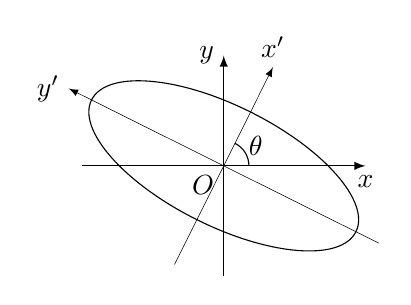
\begin{tikzpicture}[>=latex,scale=0.4]
  \draw[thin,->](-4.5,0)--(4.5,0)node[below]{$x$};
  \draw[thin,->](0,-3.5)--(0,3.5)node[left]{$y$};
  \tkzDefPoints{0/0/O,1/0/x}
  \tkzDefPointBy[rotation=center O angle 63.5](x)\tkzGetPoint{x'}
  \tkzMarkAngle[size=0.8](x,O,x')
  \tkzLabelAngle[pos=1.2](x,O,x'){$\theta$}
  \tkzLabelPoints[below left](O)
  \begin{scope}[rotate=63.5]
    \draw[very thin,->](-3.5,0)--(3.5,0)node[above]{$x'$};
    \draw[very thin,->](0,-5.5)--(0,5.5)node[left]{$y'$};
    \draw(0,0)ellipse(1.91 and 4.69);
  \end{scope}
\end{tikzpicture}
\end{document}